
\section{Thực nghiệm}

\subsection{Quy trình cân bằng lại dữ liệu}

Trong phân đoạn ảnh thực phẩm, kết cấu bề mặt đặc biệt quan trọng vì thực phẩm dễ biến dạng khi chế biến và thường phụ thuộc nhiều vào màu sắc cùng kết cấu hơn là hình dạng. Việc gộp các lớp tương đồng về kết cấu bề mặt giúp giảm mất cân bằng lớp và tạo điều kiện cho mô hình học đặc trưng thị giác vững chắc.

Vào 2023, Cote và cộng sự đã tiến hành nghiên cứu tầm quan trọng của việc khai thác dữ liệu vân của một tập dữ liệu gạch mosaic đa dạng. Kết quả cho thấy rằng kết cấu bề mặt là đặc trưng then chốt để phân biệt các vùng, đồng thời chỉ ra hạn chế của tập dữ liệu cũ và lợi ích vượt trội khi khai thác vân trong học sâu cho phân đoạn ngữ nghĩa. Vì tập dữ liệu về thực phẩm, tương tự, có đặc trưng kết cấu bề mặt đa dạng, nên kỹ thuật phân tích về vân được áp dụng với hy vọng mang lại hiệu quả tương tự.

Cụ thể, để kiểm tra và xác nhận mức độ tương đồng về kết cấu bề mặt giữa các lớp con trước khi gộp, phương pháp phân tích texture dựa trên ma trận đồng xuất hiện mức xám (Gray-Level Co-occurrence Matrix - GLCM) – một descriptor thống kê kinh điển do Haralick và cộng sự đề xuất – được áp dụng \cite{haralick1973}. GLCM mô tả phân bố không gian của các giá trị mức xám trong vùng ảnh, từ đó trích xuất các đặc trưng texture chính: contrast (độ tương phản), homogeneity (độ đồng nhất), energy (năng lượng) và correlation (tương quan). Vector đặc trưng texture trung bình \(\mathbf{f}_k\) của mỗi lớp con \(k\) được tính từ các patch ảnh thuộc lớp đó. Độ tương đồng giữa hai lớp con \(i\) và \(j\) được định lượng bằng cosine similarity trên vector đặc trưng này:$\text{Sim}(i,j) = \frac{\mathbf{f}_i \cdot \mathbf{f}_j}{\|\mathbf{f}_i\| \ \|\mathbf{f}_j\|}$

Các lớp con chỉ được gộp khi \(\text{Sim}(i,j) \geq 0.85\), đảm bảo tính thống nhất cao về vân và màu sắc bề mặt, từ đó giảm đáng kể mất cân bằng lớp và tăng kích thước mẫu huấn luyện hiệu quả cho từng lớp đích mà vẫn giữ nguyên giá trị ngữ nghĩa cốt lõi.

\begin{figure}[H]
    \centering
    \begin{subfigure}{0.48\linewidth}
        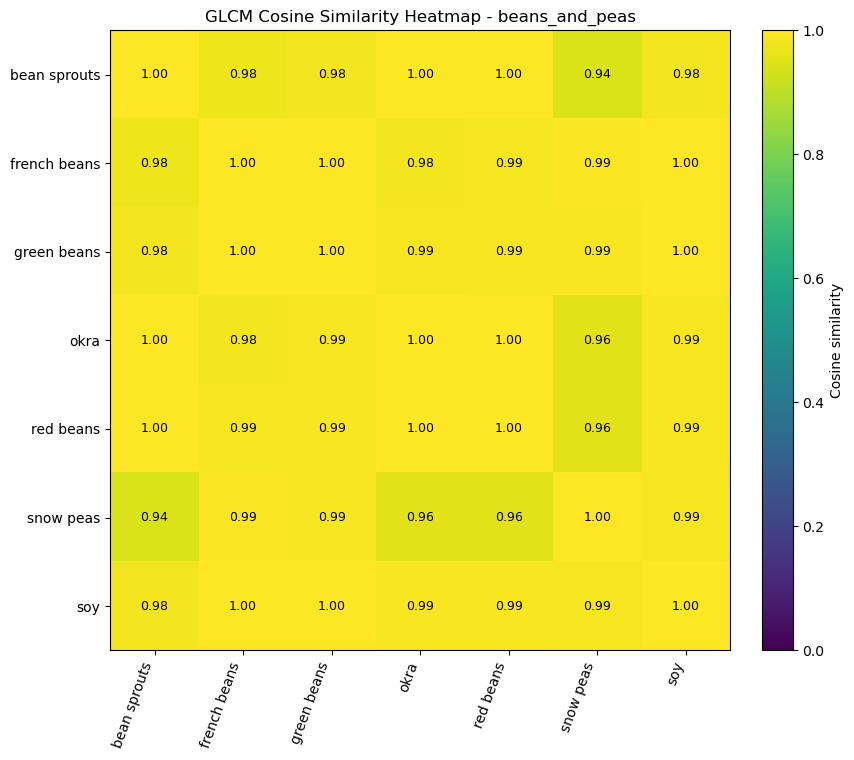
\includegraphics[width=\linewidth]{img/analyze/bean_.png}
        \caption{Beans and Peas}
    \end{subfigure}
    \begin{subfigure}{0.48\linewidth}
        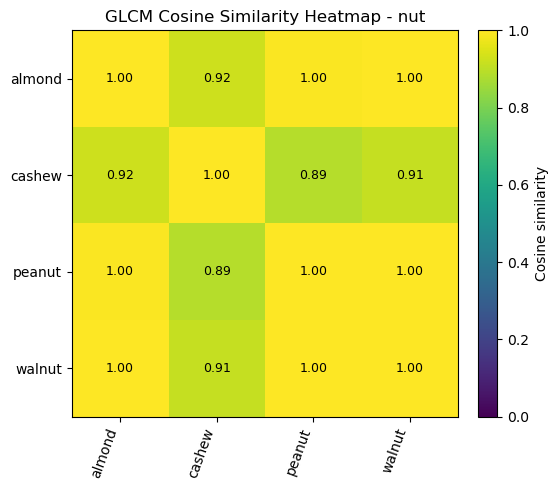
\includegraphics[width=\linewidth]{img/analyze/nut.png}
        \caption{Nuts}
    \end{subfigure}
    \caption{Ma trận cosine similarity dựa trên đặc trưng GLCM giữa các lớp con.}
\end{figure}

Quy trình tái cấu trúc dữ liệu trên bộ dữ liệu FoodSeg103 không chỉ giảm độ phân mảnh nhãn mà còn tạo điều kiện cho mô hình học được đặc trưng thị giác vững chắc hơn. Cụ thể, các nhóm lớp được gộp lại khi chúng chia sẻ đặc trưng thống nhất: ví dụ, các loại nấm khác nhau được gộp thành \texttt{mushroom} nhờ cách thức chế biến giống nhau, dẫn đến sự tương đồng cao về màu sắc và vân bề mặt.

\begin{table}[H]
\centering
\caption{Các nhóm lớp được gộp theo ngữ nghĩa và đặc trưng kết cấu bề mặt}
\label{tab:merge_groups}
\begin{tabular}{p{0.5\linewidth}p{0.29\linewidth}}
\toprule
\textbf{Nhóm lớp gốc} & \textbf{Lớp sau khi gộp} \\
\midrule
king oyster mushroom, oyster mushroom, enoki mushroom, white button mushroom, shiitake 
& \texttt{mushroom} \\
\midrule
green beans, french beans, snow peas, bean sprouts, soy, red beans, okra 
& \texttt{beans\_and\_peas} \\
\midrule
peanut, almond, cashew, walnut 
& \texttt{nut} \\
\midrule
cake, biscuit, pudding, egg tart, candy, chocolate, popcorn 
& \texttt{desserts} \\
\midrule
lemon, orange 
& \texttt{citrus} \\
\midrule
spring onion, onion, garlic, ginger 
& \texttt{alliums\_and\_garlic} \\
\midrule
cabbage, rape, lettuce 
& \texttt{leafy\_greens} \\
\midrule
kelp, seaweed
& \texttt{seaweed} \\
\bottomrule
\end{tabular}
\end{table}

Các lớp có tần suất rất thấp hoặc không đủ đặc trưng vân/màu sắc riêng biệt được ánh xạ vào lớp bao quát \texttt{other ingredients}. 

Cách tiếp cận này không chỉ giảm số lớp từ 103 xuống còn 75 mà còn tăng đáng kể kích thước mẫu huấn luyện hiệu quả cho từng lớp đích, hạn chế mất mát thông tin so với việc loại bỏ hoàn toàn. Kết quả phân tích texture cho thấy sự gộp dựa trên GLCM và cosine similarity đã tạo ra các lớp đích có tính đồng nhất cao, phù hợp với đặc trưng của thực phẩm thực tế và nâng cao khả năng khái quát hóa của mô hình phân đoạn.
\subsection{Dữ liệu sau xử lý}

Không gian nhãn giảm từ 103 xuống 75 lớp, tập dữ liệu mới sẽ được đặt là \texttt{FoodSeg103\_rebalanced}. Về số lượng ảnh, tập train giảm từ 3982 xuống 3981 ảnh (giảm 1 ảnh) và tập test giữ nguyên 2135 ảnh. Theo thống kê export trong notebook, ảnh bị loại chủ yếu do lỗi hỏng tệp ảnh (bad image), trong khi số ảnh bị loại do empty mask sau ánh xạ là 0 ở cả hai split.

\begin{table}[H]
    \centering
    \caption{So sánh dữ liệu trước và sau xử lý}
    \begin{tabular}{lrr}
        \toprule
        Chỉ số & Trước xử lý & Sau xử lý \\
        \midrule
        Số lớp mục tiêu & 103 & 75 \\
        Số ảnh train & 3982 & 3981 \\
        Số ảnh test & 2135 & 2135 \\
        \bottomrule
    \end{tabular}
\end{table}

\begin{figure}[H]
    \centering
    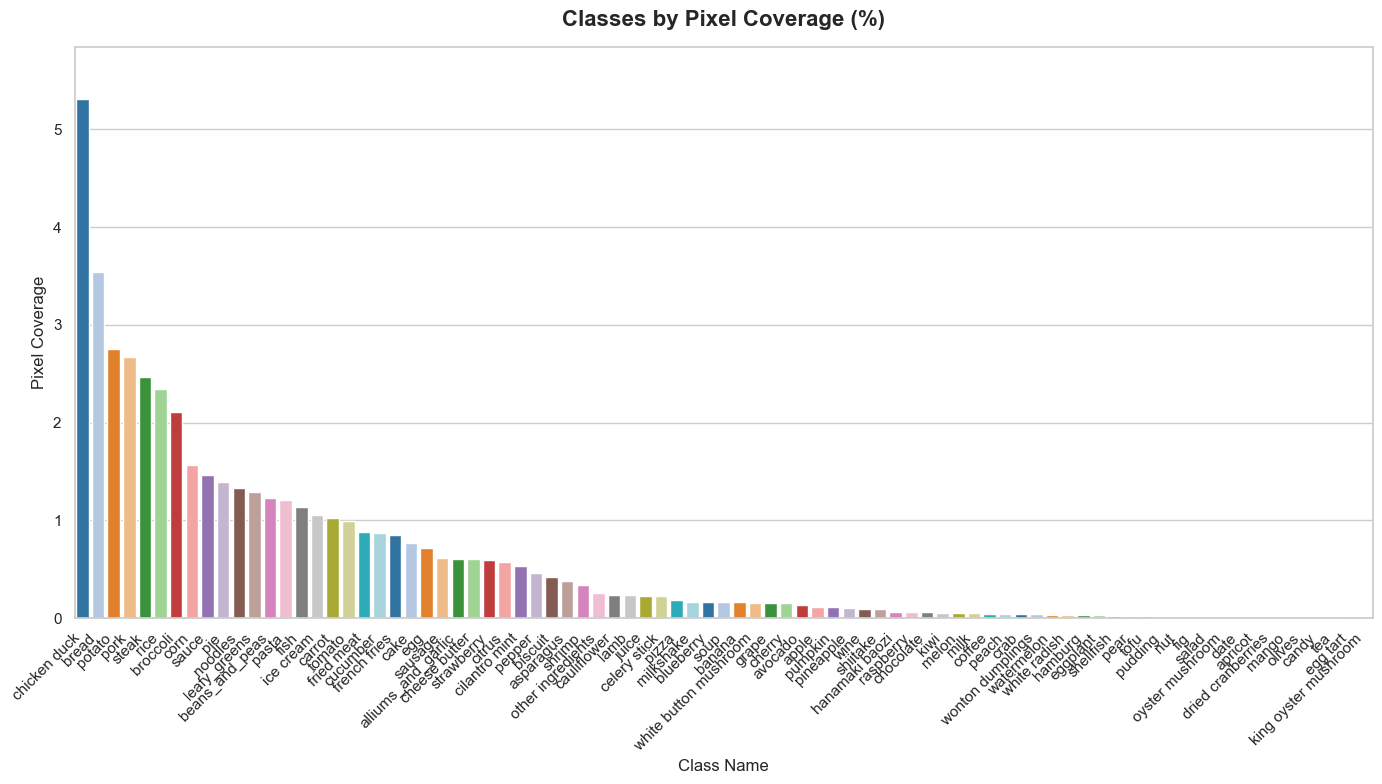
\includegraphics[width=\linewidth]{img/analyze/graph_after.png}
    \caption{Mức bao phủ pixel theo lớp sau khi gộp.}
\end{figure}

Từ góc nhìn huấn luyện, bộ \texttt{FoodSeg103\_rebalanced} giúp giảm áp lực học trên các lớp cực hiếm và tăng tính ổn định của tối ưu hóa. Tuy nhiên, long-tail chưa biến mất hoàn toàn, nên các kỹ thuật như \emph{focal loss}, \emph{class-weighted loss}, cùng theo dõi \emph{per-class IoU} vẫn là cần thiết để bảo đảm mô hình không thiên lệch về lớp đa số.

\subsection{Huấn luyện}

Trong thiết lập thực nghiệm, tập \texttt{test} của bộ \texttt{FoodSeg103\_rebalanced} được giữ nguyên để làm tập đánh giá cuối cùng, gồm 2{,}135 ảnh. Từ 3{,}981 ảnh của tập \texttt{train} sau xử lý, dữ liệu được chia tiếp thành tập huấn luyện và tập kiểm định nội bộ theo tỉ lệ 90/10 bằng hàm \texttt{train\_test\_split} với \texttt{random\_state} cố định theo seed của thí nghiệm. Theo cấu hình này, mô hình được huấn luyện trên 3{,}582 ảnh và được theo dõi trên 399 ảnh validation. Cách chia này giúp tách rõ ba vai trò: \texttt{train} để tối ưu tham số, \texttt{validation} để theo dõi hội tụ và chọn checkpoint, còn \texttt{test} giữ nguyên như tập đánh giá độc lập.

% Bảng 1: Cấu hình huấn luyện
\begin{table}[H]
    \centering
    \caption{Cấu hình tham số huấn luyện mô hình cơ sở BiSeNet.}
    \label{tab:bisenet-baseline-config}
    \resizebox{\columnwidth}{!}{%
    \begin{tabular}{ll}
        \toprule
        \textbf{Tham số (Hyperparameter)} & \textbf{Giá trị / Thiết lập} \\
        \midrule
        Kích thước crop đầu vào (Crop size) & $512 \times 512$ \\
        Kiến trúc mạng xương sống (Backbone) & Xception39 \\
        Hàm tối ưu (Optimizer) & SGD (Momentum = 0.9, Weight decay = $1\times10^{-4}$) \\
        Hàm mất mát (Loss function) & Cross-Entropy, auxiliary weight = 1.0 \\
        Tốc độ học khởi tạo (Initial LR) & $2.5\times10^{-2}$ với chiến lược Poly (power = 0.9) \\
        Kích thước lô (Batch size) & 8 \\
        Số epoch huấn luyện (Epochs) & 150 \\
        Tỉ lệ validation (Val ratio) & 0.1 \\
        Data augmentation scale & $\{0.75, 1.0, 1.5, 1.75, 2.0\}$ \\
        Số worker nạp dữ liệu (Num workers) & 0 \\
        Ignore index & 255 \\
        Automatic Mixed Precision (AMP) & True \\
        Resume training & True \\
        \bottomrule
    \end{tabular}}
\end{table}

\subsection{Kết quả}

Hình \ref{fig:bisenet-train-val-loss} trình bày diễn biến hàm mất mát trong quá trình huấn luyện BiSeNet trên toàn bộ tập \texttt{train} của bộ \texttt{FoodSeg103\_rebalanced}, với tập \texttt{validation} được tách nội bộ từ tập huấn luyện theo tỉ lệ 10\%. Đường cong cho thấy loss huấn luyện giảm dần theo epoch, trong khi loss kiểm định có giai đoạn dao động mạnh ở khoảng giữa quá trình học trước khi ổn định trở lại. Quan sát này phù hợp với đặc tính long-tail và độ khó cao của dữ liệu thực phẩm fine-grained, đồng thời cho thấy việc theo dõi validation loss là cần thiết để chọn checkpoint phù hợp thay vì chỉ dựa trên train loss.

\begin{figure}[H]
    \centering
    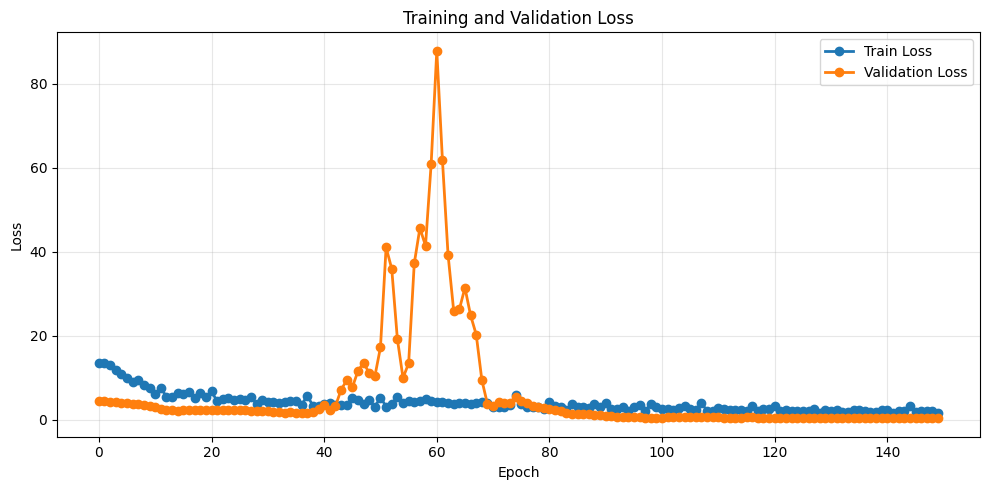
\includegraphics[width=\linewidth]{img/outputs/train-val.png}
    \caption{Diễn biến train loss và validation loss trong quá trình huấn luyện BiSeNet trên tập \texttt{train} của \texttt{FoodSeg103\_rebalanced}.}
    \label{fig:bisenet-train-val-loss}
\end{figure}

Hình \ref{fig:bisenet-output-samples} minh họa một số kết quả dự đoán của mô hình cơ sở trên tập kiểm định. Nhìn chung, BiSeNet có thể tái tạo tương đối tốt cấu trúc tổng thể của món ăn và nhận diện được các vùng nguyên liệu lớn, nhưng vẫn xuất hiện sai lệch ở các vùng biên mỏng hoặc các thành phần có texture gần nhau. Một ví dụ lỗi điển hình được trình bày ở Hình \ref{fig:bisenet-predict-problem}, trong đó mô hình dự đoán sai đáng kể ở các vùng nguyên liệu chồng lấp và có màu sắc tương tự.

\begin{figure}[H]
    \centering
    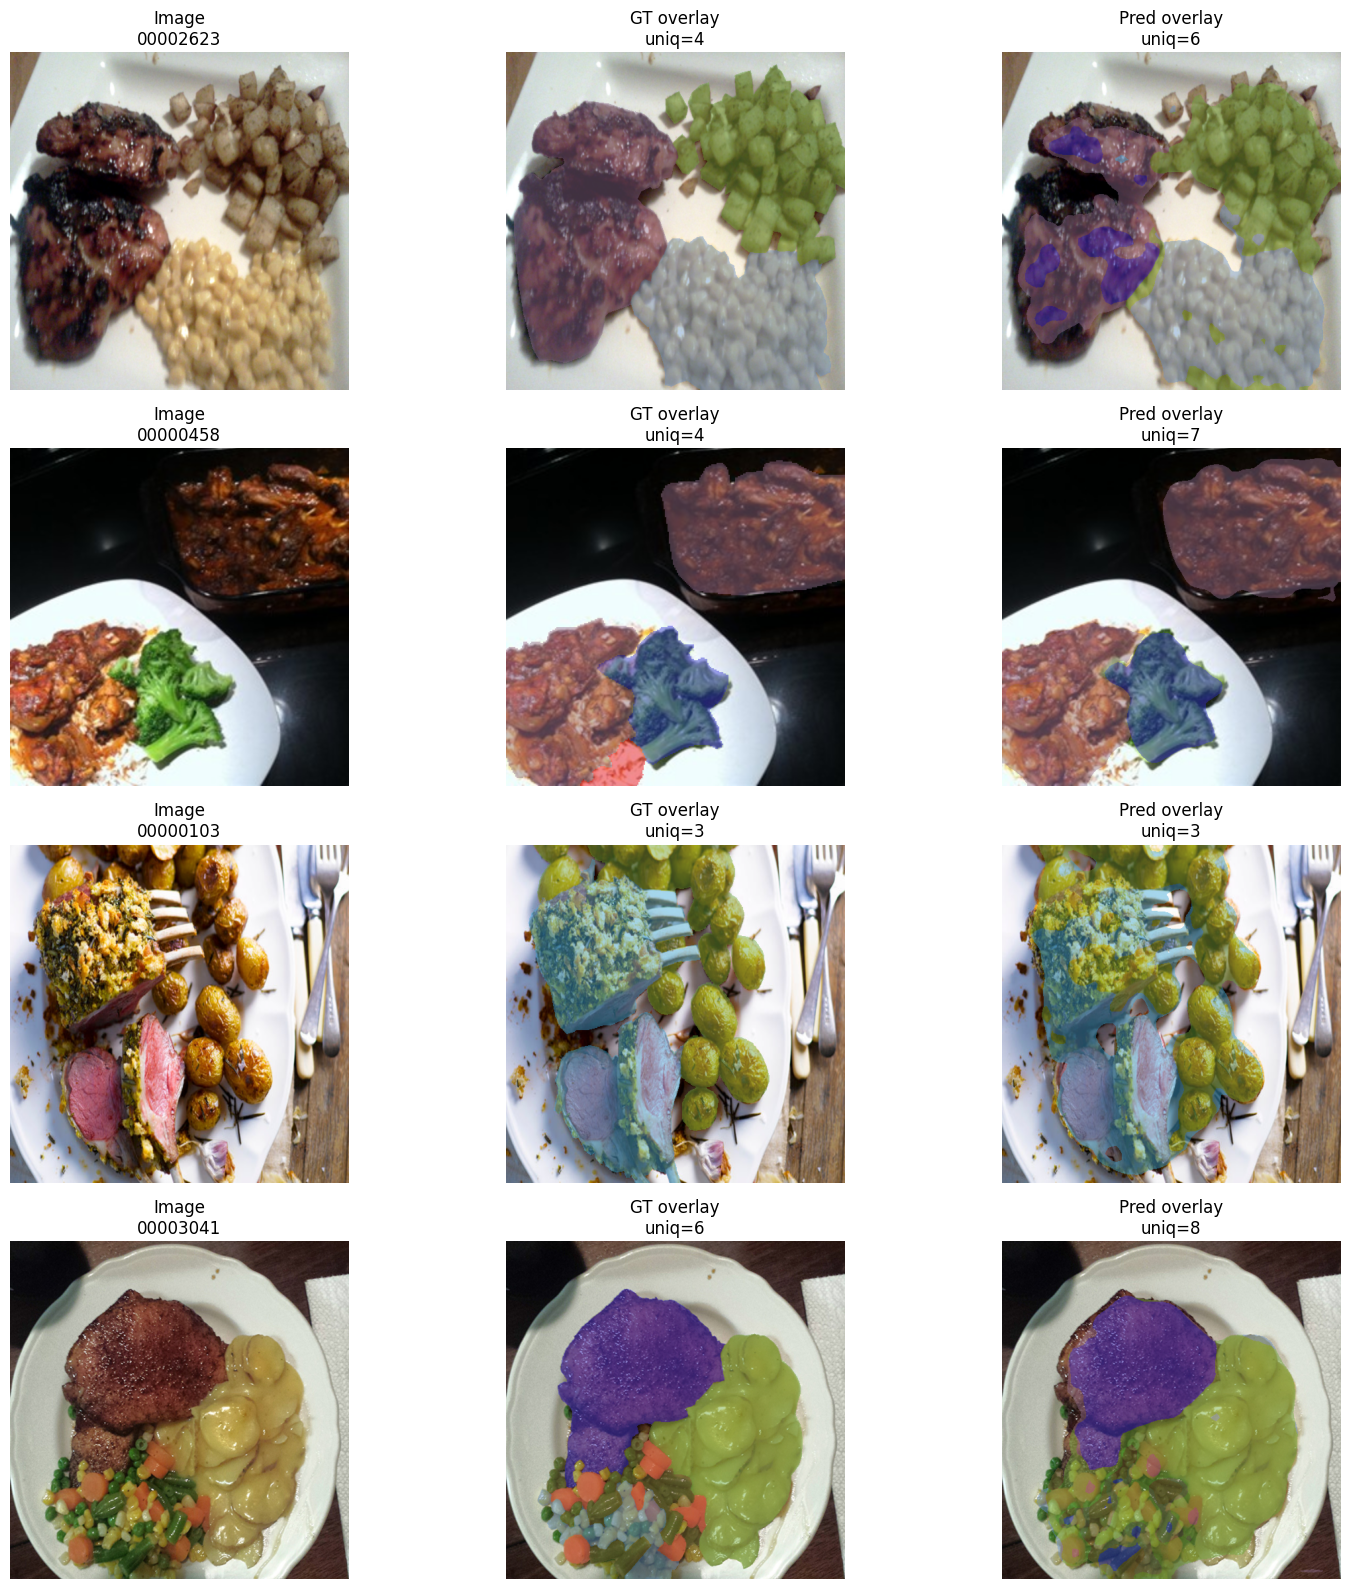
\includegraphics[width=\linewidth]{img/outputs/output-sample.png}
    \caption{Một số ví dụ dự đoán của BiSeNet trên tập kiểm định, gồm ảnh gốc, ground truth overlay và prediction overlay.}
    \label{fig:bisenet-output-samples}
\end{figure}

\begin{figure}[H]
    \centering
    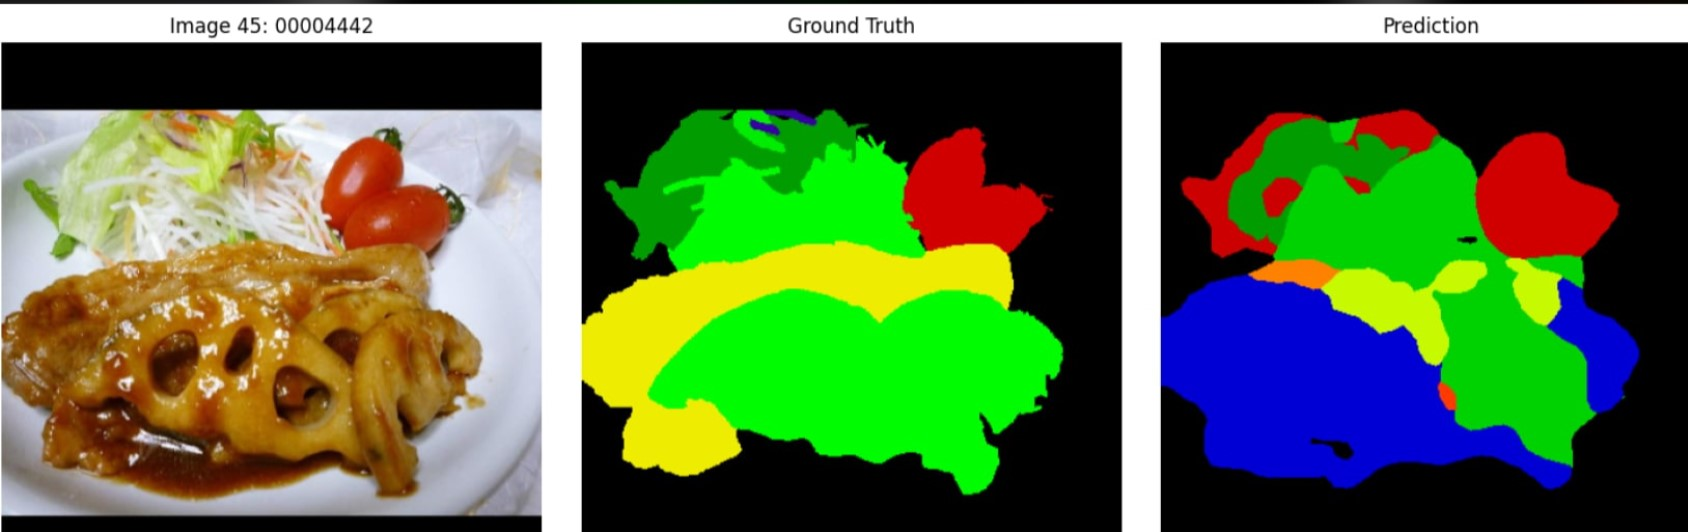
\includegraphics[width=\linewidth]{img/outputs/predict-problem.jpg}
    \caption{Ví dụ lỗi dự đoán điển hình của BiSeNet khi các thành phần nguyên liệu có ranh giới mờ hoặc chồng lấp mạnh.}
    \label{fig:bisenet-predict-problem}
\end{figure}



% Bảng 2: Kết quả đánh giá tổng thể
\begin{table}[H]
    \centering
    \caption{Các chỉ số đánh giá của mô hình cơ sở BiSeNet trên tập kiểm định của bộ dữ liệu FoodSeg103.}
    \label{tab:bisenet-baseline-results}
    \footnotesize
    \begin{tabular}{lc}
        \toprule
        \textbf{Chỉ số} & \textbf{Giá trị} \\
        \midrule
        aAcc & 0.8502 \\
        mIoU$_{\mathrm{present}}$ & 0.6354 \\
        mIoU$_{\mathrm{fg,present}}$ & 0.5828 \\
        mAcc$_{\mathrm{present}}$ & 0.7397 \\
        mAcc$_{\mathrm{fg,present}}$ & 0.6992 \\
        \bottomrule
    \end{tabular}
\end{table}

Theo tiêu chí đã định nghĩa ở phần trước, \textbf{mIoU} là chỉ số đánh giá chính vì phản ánh trực tiếp mức giao nhau trên hợp giữa mask dự đoán và ground truth ở cấp độ pixel. Trên các lớp thực sự xuất hiện trong tập đánh giá, baseline BiSeNet đạt $\mathrm{mIoU}_{\mathrm{present}} = 0.6354$. Khi chỉ xét các lớp foreground xuất hiện và loại bỏ ảnh hưởng của nền, kết quả giảm xuống còn $\mathrm{mIoU}_{\mathrm{fg,present}} = 0.5828$, cho thấy bài toán phân đoạn nguyên liệu vẫn khó đáng kể ở những vùng mang tính fine-grained.

Các chỉ số bổ sung cũng cho thấy cùng một xu hướng. Mô hình đạt $\mathrm{mAcc}_{\mathrm{present}} = 0.7397$ và $\mathrm{mAcc}_{\mathrm{fg,present}} = 0.6992$, tức là khả năng nhận diện đúng theo lớp ở mức chấp nhận được nhưng vẫn suy giảm khi chỉ xét riêng các lớp nguyên liệu foreground. Trong khi đó, $\mathrm{aAcc} = 0.8502$ tương đối cao, phản ánh rằng mô hình dự đoán đúng trên phần lớn pixel toàn cục. Tuy nhiên, do \textit{overall accuracy} dễ bị chi phối bởi các vùng lớn hoặc dễ phân đoạn, chỉ số này không đủ để thay thế mIoU trong bối cảnh dữ liệu mất cân bằng lớp và có nhiều vùng biên phức tạp như FoodSeg103.

Kết hợp giữa định lượng và quan sát trực quan, có thể thấy baseline BiSeNet đã học được cấu trúc tổng thể của món ăn và các vùng nguyên liệu lớn, nhưng vẫn gặp khó ở các thành phần có diện tích nhỏ, biên yếu hoặc texture gần nhau. Điều này phù hợp với giả thuyết của nghiên cứu: một kiến trúc lightweight có thể tạo mốc hiệu năng hữu ích, nhưng để cải thiện thêm trên bài toán ingredient-level fine-grained thì cần các cơ chế tăng cường local detail, texture hoặc boundary-aware ở các bước tiếp theo.


